% 例 3：中位线嵌套 △ABC, BC=16; D=AB中点, E=AC中点; F=AD中点, G=AE中点
\documentclass[tikz,border=4pt]{standalone}
\usepackage{ctex}
\usepackage{amsmath}
\usetikzlibrary{calc}
\begin{document}
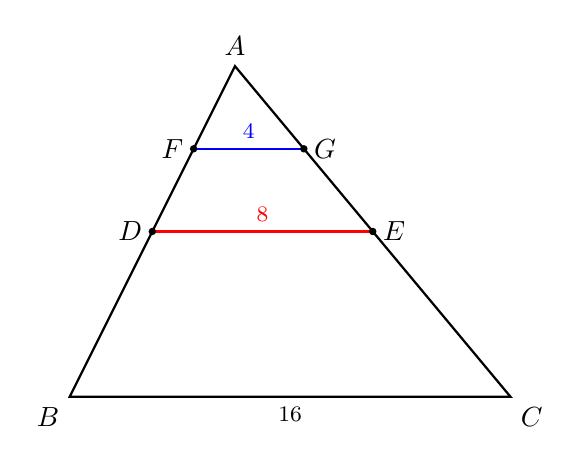
\begin{tikzpicture}[scale=0.7, thick]
  \coordinate (A) at (3,6);
  \coordinate (B) at (0,0);
  \coordinate (C) at (8,0);
  \coordinate (D) at ($(A)!0.5!(B)$);
  \coordinate (E) at ($(A)!0.5!(C)$);
  \coordinate (F) at ($(A)!0.5!(D)$);
  \coordinate (G) at ($(A)!0.5!(E)$);

  \draw (A)--(B)--(C)--cycle;
  \draw[red] (D)--(E);
  \draw[blue, thick] (F)--(G);

  \foreach \pt in {D,E,F,G} \filldraw (\pt) circle (1.3pt);

  \node[above]       at (A) {$A$};
  \node[below left]  at (B) {$B$};
  \node[below right] at (C) {$C$};
  \node[left]        at (D) {$D$};
  \node[right]       at (E) {$E$};
  \node[left]        at (F) {$F$};
  \node[right]       at (G) {$G$};
  \node[below] at ($(B)!0.5!(C)$) {\footnotesize $16$};
  \node[above, red] at ($(D)!0.5!(E)$) {\footnotesize $8$};
  \node[above, blue] at ($(F)!0.5!(G)$) {\footnotesize $4$};
\end{tikzpicture}
\end{document}
